\section{Softwarearchitektur und Signalverarbeitung}
\label{sec:software}
    Um die vom \acf{AFE} erfassten Muskelaktivitäten in präzise Steuerbefehle für die Handprothese zu übersetzen, bedarf es einer performanten Softwarearchitektur auf dem Mikrocontroller. Dieser Abschnitt beschreibt die softwareseitige Implementierung auf dem \textsf{Teensy~4.1}. Die Architektur unterteilt sich im Wesentlichen in die hardwarenahe Datenakquisition über \ac{SPI}, die digitale Signalaufbereitung mittels Frequenzfiltern sowie die anschließende Feature-Extraktion und Klassifikation.
    \subsection{Datenakquisition und Firmware-Anpassungen}
    \label{subsec:firmware_main}
        Die Basis der Signalverarbeitung bildet die Abfrage des \ac{AFE}. Während im Vorsemester ein \textsf{ADS1294} eingesetzt wurde, bei dem firmwareseitig vier Kanäle aktiv ausgelesen wurden und vier über \ac{SPI} gesendete Dummy-Pakete verworfen wurden, erfolgt in der neuen Version der vollständige Umstieg auf den \textsf{ADS1298}. Damit einhergehend wurde die zentrale Firmware so erweitert, dass nun alle acht verfügbaren Kanäle parallel erfasst und verarbeitet werden.

        Die Kernlogik der Datenaufnahme basiert auf einem interruptgesteuerten System, um eine konstante Abtastrate von $f_S = 1000$\,Hz zu garantieren. Sobald das \ac{AFE} eine Wandlung abgeschlossen hat, zieht es die \texttt{DRDY}-Leitung (Data Ready) auf \textit{LOW}. Dies löst auf dem \textsf{Teensy~4.1} direkt einen Hardware-Interrupt aus, welcher die Abfrage der Daten in der Hauptschleife initiiert. Innerhalb der Schleife werden über den \ac{SPI}-Bus mit einer Frequenz von 1\,MHz insgesamt neun Datenpakete mit jeweils 24 Bit (Status-Byte sowie acht Kanal-Bytes) seriell übertragen. Direkt nach dem Einlesen werden die 24-Bit-Werte mittels Sign-Extension in 32-Bit \texttt{int32\_t} umgewandelt. Anschließend werden die Rohwerte mit einem konstanten Faktor multipliziert, um den Messwert in Mikrovolt (\textmu V) darzustellen:
        \begin{equation*}
            \text{Messwert\,(\textmu V)} = \text{RawValue} \cdot 0,0397 \text{\,\textmu V}
        \end{equation*}
        Für die optionale Datenerfassung auf dem PC, sowie die Echtzeitvisualisierung wurde die bereits vorhandene serielle USB-Schnittstelle (betrieben bei 2.000.000 Baud) verwendet. Diese wurde firmwareseitig so skaliert, dass anstelle der ursprünglichen vier Kanäle nun die bereinigten Daten aller acht Kanäle synchronisiert auf der seriellen Schnittstelle ausgegeben werden.

        Wie bereits in \autoref{subsec:HW_kanalerweiterung} erwähnt, beliefen sich die in diesem \autoref{subsec:firmware_main} erwähnten Anpassungen gegenüber der Software des Vorsemesters lediglich auf die Erhöhung einzelner Kanalanzahl-Konstanten von vier auf acht.


    \subsection{Digitale Filterung auf dem Mikrocontroller}
        \label{subsec:biquad_filter}
        Bevor die akquirierten Daten über die Serielle Schnittstelle ausgegeben, oder in einem Ringpuffer für die Klassifikation gespeichert werden, durchlaufen sie eine digitale Filterkaskade um die Rohdaten von Störanteilen zu befreien. Die Ziele bestehen zum einen in der Entfernung des 50\,Hz-Netzbrummens sowie dessen Harmonischen und zum anderen in einer Hochpassfilterung, um niederfrequente Bewegungsartefakte zu eliminieren und die Signale um null zu zentrieren. Während im Vorsemester lediglich eine mathematische Baseline-Korrektur mittels eines Hochpassfilters erster Ordnung stattfand, wurde die Signalverarbeitungskette in der aktuellen Firmware um eine kaskadierte Biquad-Filterstruktur erweitert. Die Filterpipeline operiert bei einer Abtastrate von 1000\,Hz auf allen acht Kanälen und setzt sich aus den folgenden vier Stufen zusammen:
        \begin{itemize}[leftmargin=35px]
            \item[1.] \textbf{Hochpassfilter (15\,Hz):} Dämpft niederfrequente Bewegungsartefakte.
            \item[2.] \textbf{Notch-Filter (50\,Hz):} Eliminiert das dominante Netzbrummen der Umgebungselektronik.
            \item[3./4.] \textbf{Notch-Filter (100\,Hz \& 200\,Hz):} Unterdrückt gezielt die ersten beiden harmonischen Oberschwingungen des Netzbrummens.
        \end{itemize}
        Die mathematische Umsetzung erfolgt online direkt innerhalb der Datenerfassungsprozedur über die Differenzengleichung eines Direct-Form-I-Biquads:
        \begin{equation*}
            y[n] = b_0 \cdot x[n] + b_1 \cdot x[n-1] + b_2 \cdot x[n-2] + a_1 \cdot y[n-1] + a_2 \cdot y[n-2]  
        \end{equation*}
        \begin{figure}
            \centering
            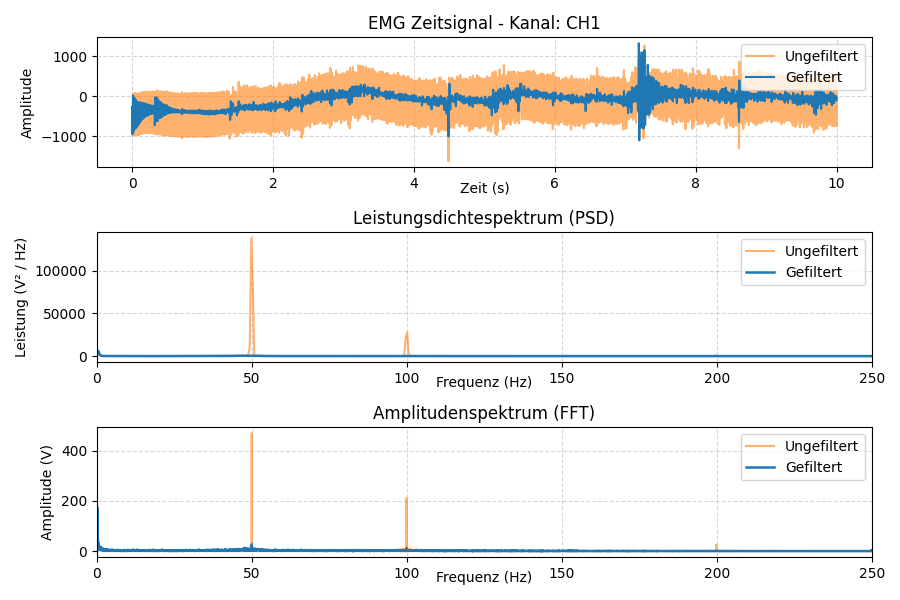
\includegraphics[width=0.85\textwidth]{figures/Filter.png}
            \caption[Vergleich von ungefiltertem und gefiltertem EMG-Signal.]{Vergleich von ungefiltertem (orange) und gefiltertem (blau) \acs{EMG}-Signal. Gut zu erkennen ist die vollständige Eliminierung des 50\,Hz-Netzbrummens sowie dessen harmonischer Oberschwingungen (100\,Hz, 200\,Hz) im Frequenzbereich.}
            \label{fig:filter}
        \end{figure}
        Die Effektivität dieser Filterkaskade lässt sich signifikant im Frequenzbereich nachweisen. Wie in \autoref{fig:filter} dargestellt, führt das ungesättigte Rohsignal im Leistungsdichte- und Amplitudenspektrum zu massiven Peaks bei 50\,Hz, 100\,Hz sowie 200\,Hz. Nach der Filterung sind diese Störlinien vollständig eliminiert, während das relevante Frequenzband des \ac{EMG}-Signals für die Merkmalsextraktion erhalten bleibt.
